\section{Same-Origin Policy}

\subsection{More on JavaScript}
User agents are client-side components responsible for the retrieval and display of web resources. Examples include \texttt{wget} and \texttt{curl}, which are command-line tools that fetch resources, as well as browsers such as Chrome and Firefox, which render web pages. In addition to displaying content, some user agents also support the execution of client-side code, such as Java Applets, ActiveX Controls, and JavaScript.

Among these, JavaScript plays a central role. It is a scripting language used to implement interactive and dynamic behavior in web pages, and it runs on the client side. To support this, browsers expose a set of APIs that allow JavaScript to interact with the web page and the browser environment. These APIs model the browser in an object-oriented manner.

\begin{minipage}{0.7\textwidth}
One key API is the Document Object Model (DOM), which provides a cross-platform and language-independent interface for representing an HTML document as a tree structure. In this model, each node in the DOM tree is an object corresponding to a part of the document. In addition, the Browser Object Model (BOM) provides APIs for interacting with browser properties. \\[3pt]
For example:

\begin{verbatim}
<html>
  <head>
  <title>Hello</title>
  </head>
  <body>
    <h1>Hello World!</h1>
    <div>
      <p>This is a paragraph.</p>
    </div>
  </body>
</html>
\end{verbatim}
\end{minipage}
\begin{minipage}{0.3\textwidth}
\begin{figure}[H]
  \centering
  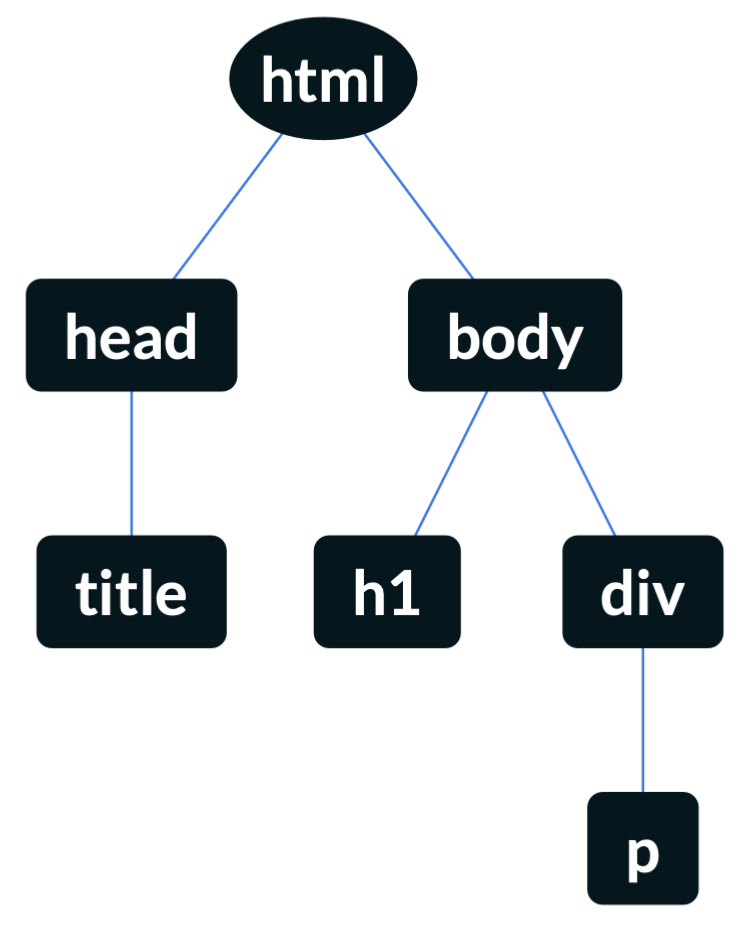
\includegraphics[width=0.9\textwidth]{Figure/DOM-1.png}
  \caption{DOM Tree}
\end{figure}
\end{minipage}

In this example, each HTML element (i.e., each tag) is represented as a DOM object. The entire document forms an \(n\)-ary tree, where each node may have multiple children accessible via the \texttt{childNodes} property. Leaf nodes, such as text or comment nodes, do not have children.

JavaScript code is typically downloaded together with the HTML page and executed on-the-fly within the context of the embedding web page. Through the DOM and BOM, JavaScript can access and modify page content, insert or delete elements, and interact with browser features such as cookies, which are critical for user session management.

Because of this powerful access, security becomes a major concern. To mitigate potential risks, browsers enforce a sandboxing mechanism for JavaScript execution. This mechanism restricts access to local files and network resources, limits certain UI behaviors (e.g., preventing very small windows), and disallows access to sensitive information such as browser history. The exact implementation of sandboxing varies across browsers.

\subsection{Same-Origin Policy}

\subsubsection{Frame Isolation}
To ensure:

- safe visit to an arbitrary web page,

- safe visit to two web pages at the same time,

- safe visit to a page embedding other frames,

we use frame isolation. Each website is isolated from all other websites, yet web pages of the same website are not isolated. We also define two types of relationships.

\textbf{Frame-Frame relationships}

- \texttt{canScript(A, B)}

This describes whether frame A can execute a script that accesses any DOM elements of frame B.

- \texttt{canNavigate(A, B)}

This describes whether frame A can change the origin of the content of frame B. 

\textbf{Frame-Principal relationships}

- \texttt{readCookie(F, D)}, \texttt{writeCookie(F, D)}

This describes whether frame F can read or write cookies of domain D. 

The Same-Origin Policy is an essential security mechanism that isolates different pages. It says a frame in one origin shall not be allowed to access resources of frames in a different origin. Then JavaScript code can access only resources that are associated with the same origin, and it cannot make HTTP requests to access the DOM, cookies, and local storage of a site or frame of a different origin. 

Here, the origin is the granularity of protection in SOP. It is a tuple of protocol, hostname, and port, and is determined by string matching. Every frame has an origin; an iframe's origin is determined by the URL where it is loaded, but not the URL of its parent frame. 

However, JavaScript code executes under the origin of the embedding frame, which introduces other problems. 

\subsubsection{HTTP Responses}
XMLHttpRequest allows JavaScript to send HTTP requests to a server and receive data in the response. However, SOP prohibits XHRs from being sent to a different origin, and JavaScript can read only responses from the same origin.

A frame can load images, CSS, and fonts from another origin. It cannot inspect the content of the resources, and it is similar to loading an iframe from another origin to ensure safety. 

A frame can also load JavaScript from another origin. It again cannot inspect the content of the script, but it can interact with it.

\subsection{Relaxing the SOP}
SOP implements security, but for origins like \texttt{www.google.com} and \texttt{google.com}, they will be treated as different origins. 

To resolve this, two frames can set their domain to the same value, i.e., \texttt{google.com}. However, the domain cannot be set to a public suffix, e.g., \texttt{com}. 

Another solution is using Cross-Origin Resource Sharing, i.e., 

\begin{verbatim}
Access-Control-Allow-Origin: http://www.foo.com
Access-Control-Allow-Origin: *
\end{verbatim}

or Cross-document messaging: 

Sender: \texttt{targetWindow.postMessage(Message, targetOrigin, [transfer])}

Receiver: \texttt{window.addEventListener("message", receiveMessage, false);}

\texttt{receiveMessage} takes an event parameter that carries the origin of the sender.